% ME 306 Course Project - Problem 16 - Group report (IEEE journal style, two-column)
\documentclass[10pt,a4paper,twocolumn]{article}
\usepackage[top=0.75in,bottom=0.9in,left=0.65in,right=0.65in,columnsep=0.24in]{geometry}
\usepackage[T1]{fontenc}
\usepackage{mathptmx}
\renewcommand{\ttdefault}{lmtt}
\usepackage{amsmath,amssymb,booktabs,graphicx,array,multirow,stfloats,adjustbox,enumitem,xcolor,cite,url}
\usepackage{tikz}\usetikzlibrary{arrows.meta,calc}
\usepackage[hidelinks]{hyperref}
\usepackage{titlesec,caption}
% ---- IEEE-like typography ------------------------------------------------------
\renewcommand{\thesection}{\Roman{section}}
\renewcommand{\thesubsection}{\Alph{subsection}}
\titleformat{\section}{\centering\normalsize\scshape}{\thesection.}{0.5em}{}
\titleformat{\subsection}{\normalsize\itshape}{\thesubsection.}{0.5em}{}
\titlespacing*{\section}{0pt}{1.0ex plus .5ex}{0.6ex}
\titlespacing*{\subsection}{0pt}{0.8ex plus .3ex}{0.3ex}
\captionsetup{font=footnotesize,labelsep=period,justification=centering}
\captionsetup[table]{labelformat=simple,textfont=sc,labelfont=sc}
\renewcommand{\thetable}{\Roman{table}}
\setlength{\parindent}{1em}\setlength{\parskip}{0pt}
\setlist{leftmargin=1.2em,itemsep=0pt,topsep=2pt}
\renewcommand{\arraystretch}{1.05}
\newcommand{\finPR}{16}
\newcommand{\finTITC}{1400}
\newcommand{\finTITK}{1673}
\newcommand{\finX}{0.30}
\newcommand{\finE}{11.9}
\newcommand{\finEps}{0.85}
\newcommand{\finEta}{40.5}
\newcommand{\finEtaTh}{41.1}
\newcommand{\finHR}{8,885}
\newcommand{\finLCOE}{11.34}
\newcommand{\finCO}{0.439}
\newcommand{\finNOx}{29.6}
\newcommand{\finFI}{1.29}
\newcommand{\finXd}{4.43}
\newcommand{\finPsi}{39.4}
\newcommand{\finMair}{237.6}
\newcommand{\finMfuel}{4.78}
\newcommand{\finMh}{0.244}
\newcommand{\finCapex}{534}
\newcommand{\finWnet}{427}
\newcommand{\finCool}{10.3}
\newcommand{\finTfive}{826}
\newcommand{\finTsix}{647}
\newcommand{\finTfour}{879}
\newcommand{\finTtwo}{523}
\newcommand{\finArea}{15,448}
\newcommand{\finQrg}{64.9}
\newcommand{\finStore}{7.0}
\newcommand{\bcEta}{31.4}
\newcommand{\bcLCOE}{10.94}
\newcommand{\bcCO}{0.643}
\newcommand{\bcNOx}{25.0}
\newcommand{\bcCool}{15.0}
\newcommand{\bcXd}{5.19}
\newcommand{\buEta}{34.67}
\newcommand{\buLCOE}{10.03}
\newcommand{\buCO}{0.583}
\newcommand{\ngLCOE}{9.00}
\newcommand{\ngCO}{0.499}
\newcommand{\dCOpct}{32}
\newcommand{\dLpct}{3.7}
\newcommand{\abateTot}{1,967}
\newcommand{\abateHtwo}{39,254}
\newcommand{\abateCycle}{-13,473}
\newcommand{\dCOcyclepct}{22}
\newcommand{\ruEta}{37.9}
\newcommand{\ruLCOE}{12.11}
\newcommand{\ruCO}{0.469}
\newcommand{\ruNOx}{18.4}
\newcommand{\ruXd}{4.61}
\newcommand{\ruPR}{30}
\newcommand{\ruTITC}{1300}
\newcommand{\ruX}{0.30}
\newcommand{\nScan}{13,200}
\newcommand{\nScanFeas}{4,337}
\newcommand{\nFeas}{106,539}
\newcommand{\nPareto}{9,653}
\newcommand{\nDom}{0}
\newcommand{\noxK}{1.31}
\newcommand{\noxN}{1.09}
\newcommand{\lcoeLo}{10.72}
\newcommand{\lcoeHi}{11.78}
\newcommand{\parityPrice}{304}
\newcommand{\fuelShare}{86}

% ---- edit these two blocks only ------------------------------------------------
\newcommand{\RepoURL}{https://github.com/varad-padhye/ME306}
\newcommand{\TeamAuthors}{24B2246 \quad 24B2206 \quad 24B2115 \quad 24B2179 \quad 24B2261}

\newcommand{\Rs}{Rs\,}
\graphicspath{{../r5_integration/figures/}}
\newcommand{\T}[1]{../r5_integration/report/tables/#1}

\begin{document}
\twocolumn[{
\begin{center}
{\Huge Design and Multi-Objective Optimisation of a Hydrogen-Blended Gas Turbine Plant for Decarbonised Grid Power}\\[10pt]
{\normalsize ME 306 Course Project --- Problem 16 --- Team Report}\\[6pt]
{\small \TeamAuthors}\\[4pt]
{\footnotesize Code, data and figures: \url{\RepoURL}}
\end{center}
\vspace{0.6em}}]

\noindent\textbf{\textit{Abstract}---A 100\,MW natural-gas simple-cycle gas turbine is redesigned to burn hydrogen--methane blends. The five team members each designed one subsystem: compression and intercooling, the combustor and fuel blend, the turbine with reheat and blade cooling, the regenerator, and the integration of all four. Each subsystem was characterised at three levels: thermodynamic design, exergy (second-law) analysis and costing. The four modules were then combined into one constant-specific-heat cycle model, which reproduces the reference baseline (35.2\% cycle efficiency, \Rs10.03/kWh). Blade cooling, which the brief does not specify, was added from published turbine data. NSGA-II searched the eight intercooling/reheat/regeneration layouts over pressure ratio, turbine-inlet temperature, hydrogen share and regenerator effectiveness, against five objectives (efficiency, exergy destruction, levelised cost of electricity (LCOE), direct CO$_2$ and a NOx index) and six constraints covering NOx, flashback and autoignition. The search found \nFeas{} feasible designs and a Pareto set of \nPareto. TOPSIS with two normalisations, followed by a reasoned trade-off, selects an \textbf{intercooled--regenerative cycle at pressure ratio \finPR, turbine-inlet temperature \finTITC\,\textdegree C, \finX{} hydrogen by volume (\finE\% of the fuel energy) and regenerator effectiveness \finEps}. It reaches \finEta\% net efficiency, \Rs\finLCOE/kWh, \finCO\,kg CO$_2$/kWh and a NOx index of \finNOx\,ppm. Against the cooled natural-gas baseline, CO$_2$ falls by \dCOpct\% for a \dLpct\% rise in LCOE. Most of that cut comes from cycle efficiency at negative cost; the hydrogen blend costs about \Rs\abateHtwo{} per tonne of CO$_2$ avoided.}

\vspace{0.4em}
\noindent\textbf{\textit{Index Terms}---Brayton cycle, hydrogen combustion, intercooling, regeneration, reheat, blade cooling, exergy analysis, LCOE, NSGA-II, TOPSIS.}

%==================================================================================
\section{Introduction}
Dispatchable gas turbines will remain part of the Indian grid as renewable capacity grows, because they balance supply and demand. Replacing part of their natural gas with green hydrogen is one way to decarbonise them; it is promoted by India's National Green Hydrogen Mission and by programmes in Europe, the US and Japan \cite{ps}. Hydrogen burns without producing CO$_2$, but it differs from methane in ways that matter for a combustor. Its laminar flame speed is 5--7 times higher, its flammability limits are much wider, its adiabatic flame temperature is higher, and its volumetric heating value is about a third of methane's \cite{ps}. Faster flames raise the risk of flashback, hotter flames raise thermal NOx, and green hydrogen currently costs about 3.4 times more per GJ than imported natural gas.

The brief \cite{ps} asks the team to explore this trade-off with the Brayton-cycle improvements covered in class (intercooling, reheat, regeneration) and to recommend \emph{one} configuration. The recommendation must be justified on performance, exergy destruction, cost, environmental impact and operational safety. The work was split into five roles, each owning one subsystem at three levels (core design, exergy, cost) \cite{ps,plan}. This report presents the combined work: the problem and baseline (Section~\ref{sec:prob}), the team method (Section~\ref{sec:method}), the four subsystem designs (Section~\ref{sec:sub}), the integrated model and its validation (Section~\ref{sec:int}), the optimisation and selection (Sections~\ref{sec:res}--\ref{sec:sel}), the final design (Section~\ref{sec:final}), and the discussion, limitations and conclusions.

%==================================================================================
\section{Problem Definition and Baseline}\label{sec:prob}
The reference plant is deliberately the simplest possible: a 100\,MW open simple Brayton cycle on 100\% natural gas (Table~\ref{tab:base}). The brief notes that at a fixed turbine-inlet temperature (TIT), hydrogen changes the combustion side far more than the cycle side, and asks the team to verify this.

\begin{table}[!t]\centering\caption{Baseline Plant (Problem Statement)}\label{tab:base}
\footnotesize\begin{tabular}{@{}ll@{}}\toprule Parameter & Value\\\midrule
Net output; cycle & 100\,MW; simple open Brayton\\
Fuel & natural gas (CH$_4$), LHV 48\,MJ/kg; H$_2$ 0\%\\
Ambient & 35\,\textdegree C, 1.013\,bar\\
Pressure ratio; TIT & 15; 1400\,\textdegree C (1673\,K)\\
$\eta_c$ / $\eta_t$ & 0.87 / 0.90\\
Pressure losses & inlet 1\%, combustor 4\%, exhaust 1\%\\
$\eta_b$ / $\eta_{gen}$ & 0.99 / 0.985\\
Air; hot gas & $c_p$ 1.005, $\gamma$ 1.4; $c_p$ 1.15\,kJ/kg\,K, $\gamma$ 1.333\\
Economics & 9\%, 25\,y, O\&M 3\%/y, load factor 50\%\\
Fuel prices & NG \Rs850/GJ; green H$_2$ \Rs350/kg (\Rs2917/GJ)\\
Plant cost & \Rs4\,crore/MW\\
\midrule Computed: $\eta$, heat rate & 35.2\% (34.7\% net), 10\,380\,kJ/kWh\\
Computed: flows, CO$_2$, LCOE & 229/6.0\,kg/s, 0.58\,kg/kWh, \Rs10.03/kWh\\\bottomrule
\end{tabular}\end{table}

\textbf{Decision variables}: pressure ratio and intercooling (R1); hydrogen share and excess air (R2); TIT and reheat (R3); regenerator effectiveness (R4). \textbf{Objectives}: maximise efficiency, minimise exergy destruction, LCOE, direct CO$_2$ and a NOx index. \textbf{Constraints}: TIT within the firing limit of the assumed hot-section technology; a flashback margin; NOx within the CPCB limit; regeneration only where turbine exhaust is hotter than compressor delivery \cite{ps}.

%==================================================================================
\section{Team Organisation and Method}\label{sec:method}
\subsection{Roles}
R1 owned compression and intercooling, R2 the combustor and fuel blend, R3 the turbine, reheat and cooling, R4 the regenerator and exhaust heat recovery, and R5 the integration, LCOE and fuel supply, and the optimisation \cite{ps}. The four-week plan \cite{plan} was followed: Week 1 hand calculations and agreed interfaces; Week 2 modules validated against a common reference; Week 3 sweeps, exergy, cost and optimisation; Week 4 decision and reporting.

\subsection{Shared conventions}
\begin{itemize}
\item \textbf{Model}: constant-specific-heat cycle model with $h=c_pT$ for all optimisation runs, as the plan requires. Cantera (GRI-Mech 3.0) is used only for combustion quantities: flame temperature, product composition, flame speed, NOx kinetics and autoignition (R2).
\item \textbf{Hydrogen share} $x$ is the \emph{volume} (mole) fraction of H$_2$ in the fuel. The energy share $e$ is always reported alongside: $x=0.30$ supplies only $e=11.9\%$ of the fuel energy.
\item \textbf{Dead state} 308.15\,K, 1.013\,bar. All quantities are per kg of compressor-inlet air.
\item \textbf{One parameter file} (\texttt{r5\_params.py}) holds every number with its owner and source. One state numbering is used throughout (Fig.~\ref{fig:schem}).
\item Each on/off layout (intercooling, reheat, regeneration) is a separate case.
\end{itemize}

%==================================================================================
\section{Subsystem Design}\label{sec:sub}
\subsection{Compressor and Intercooling (R1)}
\emph{Core.} For isentropic efficiency $\eta_c$, $T_2=T_1[1+(r_p^{(\gamma-1)/\gamma}-1)/\eta_c]$ and $w_c=c_{p,a}(T_2-T_1)$. At $r_p=15$ this gives $T_2=721.8$\,K and $w_c=415.7$\,kJ/kg, matching the reference 722\,K \cite{r1}. For two equal stages ($r_s=\sqrt{r_p}=3.873$) with an intercooler of effectiveness $\varepsilon_{IC}$ (cooling to 35\,\textdegree C), $T_{1b}=T_{1a}-\varepsilon_{IC}(T_{1a}-T_0)$. R1's candidate $\varepsilon_{IC}=0.85$ gives $T_{1a}=475.5$, $T_{1b}=333.3$ and $T_2=514.2$\,K. Compressor work falls to 350.0\,kJ/kg ($-15.8\%$, $-15.1$\,MW) for an intercooler duty of 32.9\,MW. Work rises with pressure ratio and falls with $\varepsilon_{IC}$ (Fig.~\ref{fig:r1}, left).

\emph{Exergy.} Each compressor stage destroys 3.35\,MW. The intercooler destroys 7.57\,MW (heat rejected to the environment), against 5.55\,MW for the single-stage machine. \emph{Intercooling saves work but does not by itself reduce the subsystem's exergy destruction} \cite{r1}.

\emph{Cost.} The intercooler costs 5--8\% of the base plant, \Rs20--32\,crore (midpoint 26), or \Rs3.43\,crore/y annualised. R1 concluded that whether intercooling pays depends on the rest of the cycle. The integration confirmed this, and showed a second benefit: colder compressor delivery means less blade-cooling air (Fig.~\ref{fig:r1}, right).

\begin{figure}[!t]\centering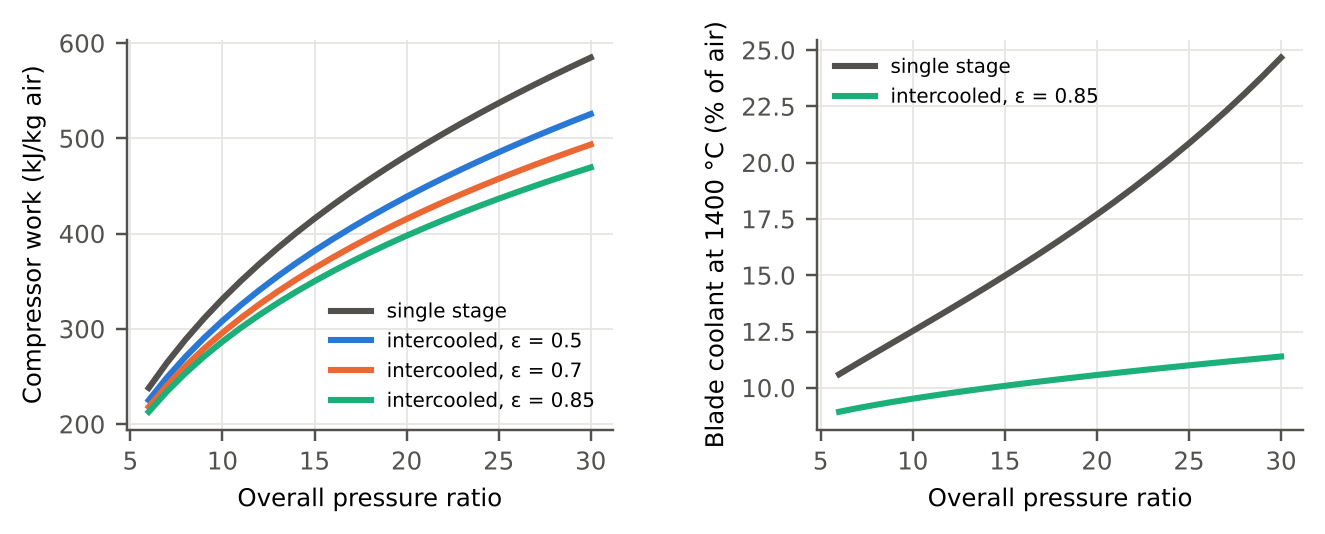
\includegraphics[width=\columnwidth]{fig_sub_R1.png}
\caption{R1: compressor work against pressure ratio (left); blade coolant needed at 1400\,\textdegree C for single-stage and intercooled delivery (right).}\label{fig:r1}\end{figure}

\subsection{Combustor and Fuel Blend (R2)}
\emph{Stoichiometry.} $(1-x)$CH$_4+x$H$_2+(2-1.5x)$(O$_2$+3.76N$_2$)$\rightarrow(1-x)$CO$_2+(2-x)$H$_2$O+N$_2$. $(A/F)_{st}$ rises from 17.13 (CH$_4$) to 34.07 (H$_2$). Because H$_2$ has a third of methane's volumetric LHV, energy share lags volume share (Fig.~\ref{fig:r2}, left) \cite{r2}.

\emph{Fuel--air ratio and gas properties.} Energy balance: $f=(c_{p,g}T_3-c_{p,a}T_2)/(\eta_bLHV-c_{p,g}T_3)=0.0263$ at baseline (Cantera 0.0257; the difference is the 48 against 50\,MJ/kg convention), giving an overall excess-air ratio of 2.22. R2 tabulated hot-gas $c_{p,g}$ and $\gamma_g$ against $x$ (1.150$\to$1.191\,kJ/kg\,K as exhaust H$_2$O rises from 8.8\% to 14.6\%). With these properties, efficiency at fixed TIT changes by only +0.72 points from $x=0$ to 1, which \emph{confirms the brief's claim}.

\emph{NOx index.} Thermal (Zeldovich) NO from Heywood's rate expression \cite{heywood} at the primary-zone temperature with Cantera equilibrium species, over 10\,ms. It is calibrated to 25\,ppm (15\% O$_2$) for natural gas at 1790\,K, cross-checked against full GRI kinetics, and behaves like Rizk--Mongia-type correlations \cite{lefebvre}. If the burner hardware is unchanged (S1), NOx reaches 411\,ppm at $x=1$. If the burner is re-tuned to the same primary-zone temperature (S2, adopted), it stays at 25--35\,ppm (Fig.~\ref{fig:r2}, centre). The CPCB band for 100--400\,MW is 75\,ppm \cite{cpcb}, equivalent to a primary zone below 1849\,K.

\emph{Flashback index.} $FI=g_c(x)/g_c(0)$, where $g_c\propto S_L^2/\alpha$ is the critical boundary-layer velocity gradient \cite{lewis}, with flame speeds from Cantera at 14.4\,bar. $FI=1.26$ at $x=0.3$, 1.94 at 0.65 and 7.0 at 1. Preheated (regenerated) air makes it worse (Fig.~\ref{fig:r2}, right). Hardware tiers: conventional DLN up to $x=0.3$; advanced premixer up to 0.65 ($FI\le2$); redesigned burner beyond.

\emph{Autoignition (new constraints found by R2).} The premixer needs an ignition delay over 15\,ms, so combustor-inlet air must stay at or below 1050\,K. A reheat combustor is stabilised by autoignition, so the hydrogen it can take is limited to $x\le0.27/0.41/0.47$ at $r_p=10/15/20$.

\emph{Exergy and cost.} Combustion destroys 30.0\% of the fuel exergy on natural gas and 27.7\% on pure H$_2$. It is the largest loss in the plant. The H$_2$-capable combustor premium is 0, 4, 9.5 and 15\% of base plant cost at $x$ = 0, 0.3, 0.65 and 1. Hydrogen storage costs \Rs55\,000 per kg of capacity, sized for 8\,h of full-load operation, from US DOE data \cite{doe}. In the baseline cycle, CO$_2$ avoided by hydrogen costs about \Rs36\,500/t.

\begin{figure*}[!t]\centering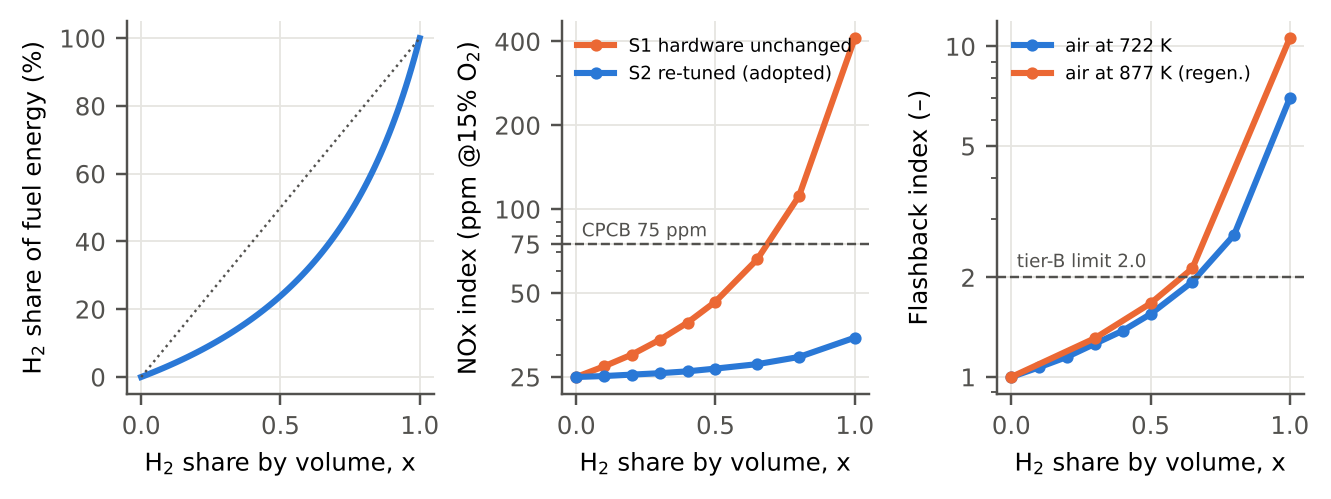
\includegraphics[width=0.92\textwidth]{fig_sub_R2.png}
\caption{R2: hydrogen energy share against volume share (left); NOx index for unchanged hardware (S1) and re-tuned burner (S2, adopted) (centre); flashback index at baseline and regenerated air temperature (right).}\label{fig:r2}\end{figure*}

\subsection{Turbine, Reheat and Blade Cooling (R3)}
\emph{Core.} $T_4=T_3[1-\eta_t(1-(p_4/p_3)^{(\gamma_g-1)/\gamma_g})]$ and $w_t=(1+f)c_{p,g}(T_3-T_4)$. At baseline, $T_4=944.6$\,K and $w_t=860.1$\,kJ/kg air \cite{r3}. Reheat expands the gas to an intermediate pressure, reheats it to TIT in a second combustor, and expands it again. Specific work rises (577 against 444\,kJ/kg), but the extra heat is added at a lower mean temperature.

\emph{Material and cooling limits.} The brief asks that TIT stay within the firing limit of an \emph{assumed} hot-section technology, but gives no numbers. These were taken from the literature:
\begin{itemize}
\item \textbf{Firing limit 1500\,\textdegree C.} Mitsubishi lists F-class at 1400\,\textdegree C and G/H-class at 1500\,\textdegree C. Only the J-class reached 1600\,\textdegree C, with steam cooling of stationary parts \cite{mhi1,mhi2}. The baseline is therefore F-class technology.
\item \textbf{Blade metal 1150\,K.} At a 1400\,\textdegree C entry, coated blades run with metal near 930\,\textdegree C \cite{cam}. CMSX-4 has been flight-qualified near 1130\,\textdegree C \cite{cmsx}. 1150\,K leaves margin for a 25-year industrial life.
\item \textbf{Coolant.} Horlock-type relation \cite{horlock}: $\phi=(T_3-T_m)/(T_3-T_2)$, $\psi=B(c_{p,g}/c_{p,a})\,\phi/[\eta_{cool}(1-\phi)]\,h_x$, with $\eta_{cool}=0.7$. The heat-transfer index $h_x$ rises 3.4\% from $x$ = 0 to 1 because of the H$_2$O-rich gas (R3, Dittus--Boelter). $B$ was calibrated to 15\% of compressor air at 1400\,\textdegree C, between R3's 12\% and the roughly 20\% (including sealing air) quoted for 1350\,\textdegree C-class machines \cite{asme}. Aero engines take 20--25\% \cite{ceas}.
\end{itemize}
Coolant is bled at compressor delivery and mixed in mid-expansion. Cooling costs about 3 points of efficiency at baseline, and reheat needs a second cooled turbine (Fig.~\ref{fig:r3}).

\emph{Exergy and cost.} Turbine destruction rises from 2.5\% to 5.6\% of fuel exergy once coolant mixing is included. Reheat hardware is 10--15\% of base (\Rs40--60\,crore). The hot-section premium is +4\% of base per 100\,K above 1400\,\textdegree C (R3 assumption).

\begin{figure}[!t]\centering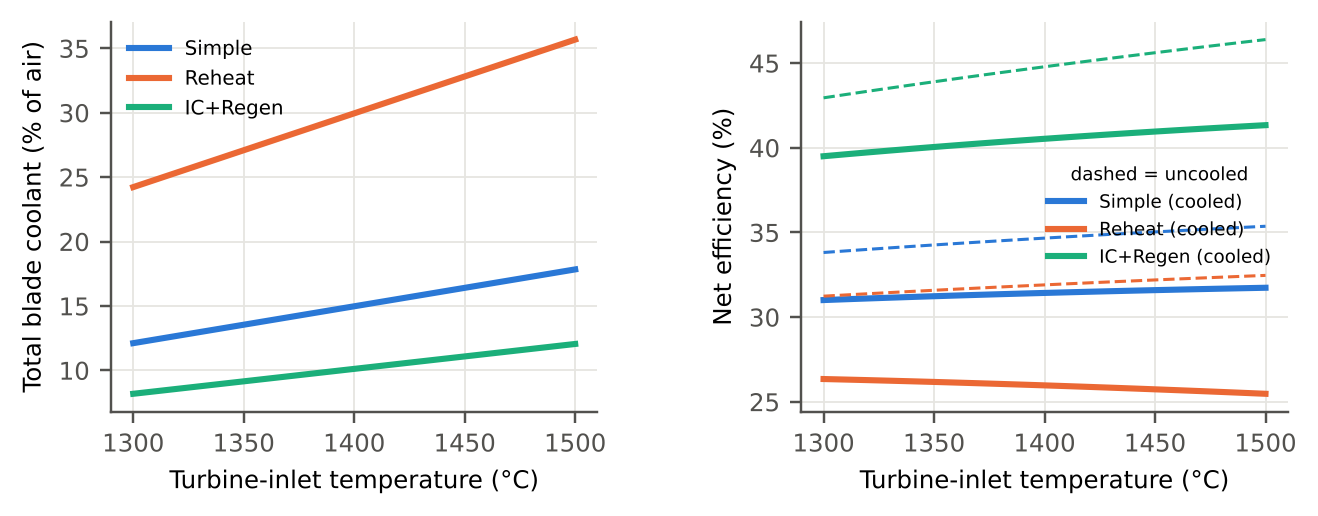
\includegraphics[width=\columnwidth]{fig_sub_R3.png}
\caption{R3: total blade coolant (left) and net efficiency, cooled (solid) and uncooled (dashed) (right), against TIT at $r_p=15$, natural gas.}\label{fig:r3}\end{figure}

\subsection{Regenerator and Exhaust Heat Recovery (R4)}
\emph{Core.} Counterflow recuperator: $\dot Q=\varepsilon C_{min}(T_4-T_2)$, $T_5=T_2+\dot Q/C_c$, $T_6=T_4-\dot Q/C_h$, allowed only if $T_4>T_2$ with both terminal approaches $\ge$20\,K. At baseline with $\varepsilon=0.75$: 38.65\,MW recovered, air preheated to 888.8\,K, exhaust cooled to 801.8\,K, net efficiency 34.7$\to$40.0\%, and 13.4\% less fuel \cite{r4}. Regeneration stops being possible near $r_p=25.5$, where $T_4\approx T_2$.

\emph{Sizing, exergy, cost.} From $\varepsilon$--NTU, $UA=576$\,kW/K, or 11\,521\,m$^2$ at $U=50$\,W/m$^2$K. Regenerator destruction is 1.17\,MW. The stack thermal exergy falls from 78.6 to 53.9\,MW. At the cost allowance (8--12\% of base), LCOE is \Rs8.97/kWh and the simple payback 0.8\,y. A 3\% pressure loss per side costs 0.9 points. Area grows steeply with $\varepsilon$, but in the integrated plant LCOE still falls up to the 0.85 screening bound (Fig.~\ref{fig:r4}).

\begin{figure*}[!t]\centering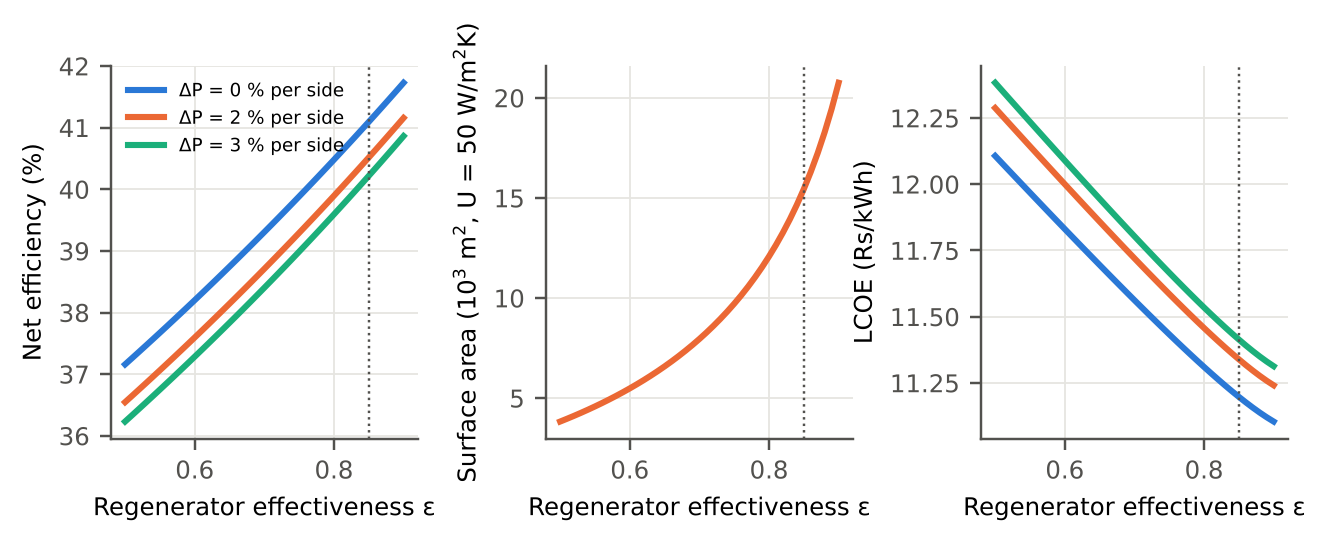
\includegraphics[width=0.92\textwidth]{fig_sub_R4.png}
\caption{R4 in the final cycle (IC + Regen, $r_p=16$, 1400\,\textdegree C, $x=0.3$): efficiency for three pressure losses (left), heat-transfer area (centre) and LCOE (right) against effectiveness. Dotted line: chosen $\varepsilon=0.85$.}\label{fig:r4}\end{figure*}

%==================================================================================
\section{Integrated Model (R5)}\label{sec:int}
\subsection{Plant, coupling and constraint models}
Fig.~\ref{fig:schem} shows the integrated plant. The regenerator, combustor and turbine are coupled: preheat changes the fuel flow, which changes the hot-side capacity rate. They are solved by fixed-point iteration on $T_4$ to $10^{-7}$\,K. Turbines use the polytropic efficiency equivalent to 0.90, so splitting an expansion at the coolant-injection point does not change its overall efficiency. The plant is sized by $\dot m_a=100\,\text{MW}/(\eta_g w_{net})$.

The constraint indicators come from R2's tables:
\begin{itemize}
\item \textbf{NOx}: R2's S2 strategy. Above 1400\,\textdegree C the primary zone keeps R2's dilution margin, $T_{pz}=1790+(T_3-1673)$\,K. Inlet-temperature and reheat-dilution terms, NOx $\propto e^{k(T_5-722)}(f_1/f_{tot})^n$ with $k=\noxK\times10^{-3}$/K and $n=\noxN$, were fitted to R2's eight-configuration table (all eight within 0.4\,ppm).
\item \textbf{Flashback}: $FI(x,T_5)$ interpolated between R2's 722\,K and 877\,K tables.
\item \textbf{Autoignition}: the 1050\,K premixer limit and the reheat $x_{max}(r_p)$ limit.
\end{itemize}

\begin{figure*}[!t]\centering
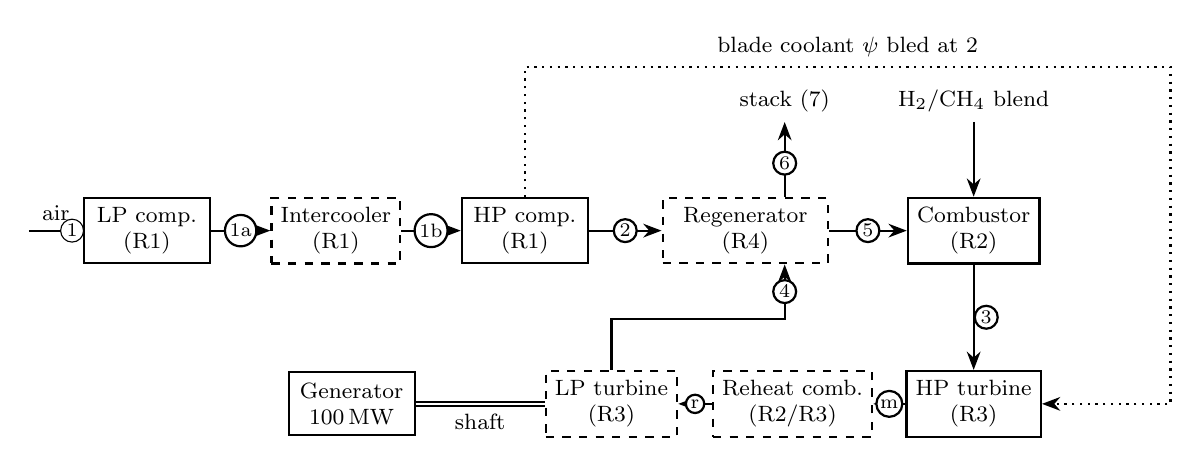
\begin{tikzpicture}[font=\footnotesize,>=Stealth,box/.style={draw,thick,minimum width=1.6cm,minimum height=0.8cm,align=center},opt/.style={box,dashed},st/.style={circle,fill=white,draw,inner sep=0.8pt,font=\scriptsize}]
\node[box] (lpc) at (0,0) {LP comp.\\(R1)};
\node[opt] (ic) at (2.4,0) {Intercooler\\(R1)};
\node[box] (hpc) at (4.8,0) {HP comp.\\(R1)};
\node[opt,minimum width=2.1cm] (rg) at (7.6,0) {Regenerator\\(R4)};
\node[box] (cc) at (10.5,0) {Combustor\\(R2)};
\node[box] (hpt) at (10.5,-2.2) {HP turbine\\(R3)};
\node[opt] (rh) at (8.2,-2.2) {Reheat comb.\\(R2/R3)};
\node[opt] (lpt) at (5.9,-2.2) {LP turbine\\(R3)};
\node[box] (gen) at (2.6,-2.2) {Generator\\100\,MW};
\draw[->,thick] (-1.5,0) -- node[above]{air} (lpc);
\draw[->,thick] (lpc) -- node[st]{1a} (ic); \draw[->,thick] (ic) -- node[st]{1b} (hpc);
\draw[->,thick] (hpc) -- node[st]{2} (rg); \draw[->,thick] (rg) -- node[st]{5} (cc);
\draw[->,thick] (cc) -- node[st,right]{3} (hpt); \draw[->,thick] (hpt) -- node[st]{m} (rh);
\draw[->,thick] (rh) -- node[st]{r} (lpt);
\draw[->,thick] (lpt.north) -- ++(0,0.65) -| node[st,pos=0.75]{4} ($(rg.south)+(0.5,0)$);
\draw[->,thick] ($(rg.north)+(0.5,0)$) -- node[st,pos=0.45]{6} ++(0,0.95) node[above]{stack (7)};
\draw[->,thick] ($(cc.north)+(0,0.95)$) node[above]{H$_2$/CH$_4$ blend} -- (cc.north);
\draw[->,dotted,thick] (hpc.north) -- ++(0,1.65) -- ++(8.2,0) node[pos=0.5,above]{blade coolant $\psi$ bled at 2} |- (hpt.east);
\node[st] at (-0.95,0) {1}; \draw[thick,double] (gen) -- node[below]{shaft} (lpt);
\end{tikzpicture}
\caption{Integrated plant with team state numbering. Dashed blocks are optional; each combination is a separate case. Without reheat, the HP turbine expands to state 4. Without regeneration, $5\equiv2$ and $6\equiv4$.}\label{fig:schem}\end{figure*}

\emph{Exergy.} Flow exergy is $\psi=c_p(T-T_0)-T_0[c_p\ln(T/T_0)-R\ln(p/p_0)]$, and fuel exergy uses Szargut ratios of 1.0366 (CH$_4$) and 0.9764 (H$_2$) \cite{szargut}. Each component's destruction is taken from its own exergy balance, so $\dot X_{fuel}=\dot W_{el}+\sum\dot X_D+\dot X_{stack}$ closes exactly (residual $10^{-13}$). The second-law efficiency is $\Psi=\dot W_{el}/\dot X_{fuel}$.

\emph{Cost and CO$_2$.} LCOE $=[C(\mathrm{CRF}+0.03)+F]/E$ with CRF $=0.1018$ and $E=438$\,GWh/y. Capital $C$ = base + intercooler 6.5\% + regenerator $\propto UA$ (\Rs40\,cr at $UA=576$\,kW/K, R4) + reheat 12.5\% + H$_2$ combustor premium + hot-section premium + H$_2$ storage. Fuel $F$ uses the energy-weighted blend price, so hydrogen \emph{supply} is carried in the delivered price. Direct CO$_2$ $=3.6/\eta_{net}\cdot(1-e)\cdot56.1$\,g/MJ; green H$_2$ is assumed to have zero upstream emissions.

\subsection{Reconciliation of the subsystem submissions}
Where the submissions differed, one team value was fixed. Intercooler $\varepsilon$ is 0.85 (R2's stand-in had used 0.9), and both the intercooler and regenerator get a 2\% pressure loss. Regenerator $\varepsilon$ is a decision variable over 0.50--0.85 (R4); R2 had used 0.70. Energy share is computed by R2's method throughout; R4's volumetric conversion gave 11.45\% against 11.9\%. Air flow is re-sized for every design. Cooling is included in every optimisation run.

\subsection{Validation}
\begin{table}[!t]\centering\caption{Validation of the Integrated Code Against the Plan and Each Subsystem}\label{tab:valid}
\scriptsize\adjustbox{max width=\columnwidth}{\input{\T{validation.tex}}}
\end{table}
With each teammate's own settings, the integrated code reproduces the plan's baseline and every hand-off (Table~\ref{tab:valid}). The only difference is R3's cooled case, by 0.2 points, because R3 additionally rescales gas properties with $f$ through Cantera.

%==================================================================================
\section{Results}\label{sec:res}
\subsection{Candidate configurations}
\begin{table*}[!t]\centering\caption{All Eight Layouts at $r_p=15$, TIT 1400\,\textdegree C, $x=0.30$, $\varepsilon=0.75$ (CO$_2$ kg/kWh, NOx ppm, $\psi_{cool}$ Coolant Fraction, $\Psi$ Second-Law Efficiency)}\label{tab:cand}
\scriptsize\input{\T{candidates.tex}}\end{table*}
Table~\ref{tab:cand} and Fig.~\ref{fig:cand} compare the layouts with and without blade cooling. Three results drive the rest of the study:
\begin{enumerate}
\item \textbf{Cooling costs about 3 points} at baseline: 15\% of the air bypasses the combustor.
\item \textbf{Reheat is penalised most}, because its LP turbine is also fired to TIT and needs coolant (30\% in total). R2's uncooled screening ranked IC+Regen+Reheat first; with cooling it falls from 43.5\% to 36\%.
\item \textbf{Intercooling becomes more valuable}: delivery at 516\,K instead of 722\,K cuts the coolant from 15\% to 10\%, and widens the regeneration margin. IC+Regen is the most efficient cooled layout.
\end{enumerate}
Fig.~\ref{fig:pr} shows that regenerative cycles prefer moderate pressure ratios and reheat cycles high ones. Raising TIT gains only about 0.9 points per 100\,K with cooling, and the NOx limit is reached near 1450\,\textdegree C (Fig.~\ref{fig:tit}).

\begin{figure*}[!t]\centering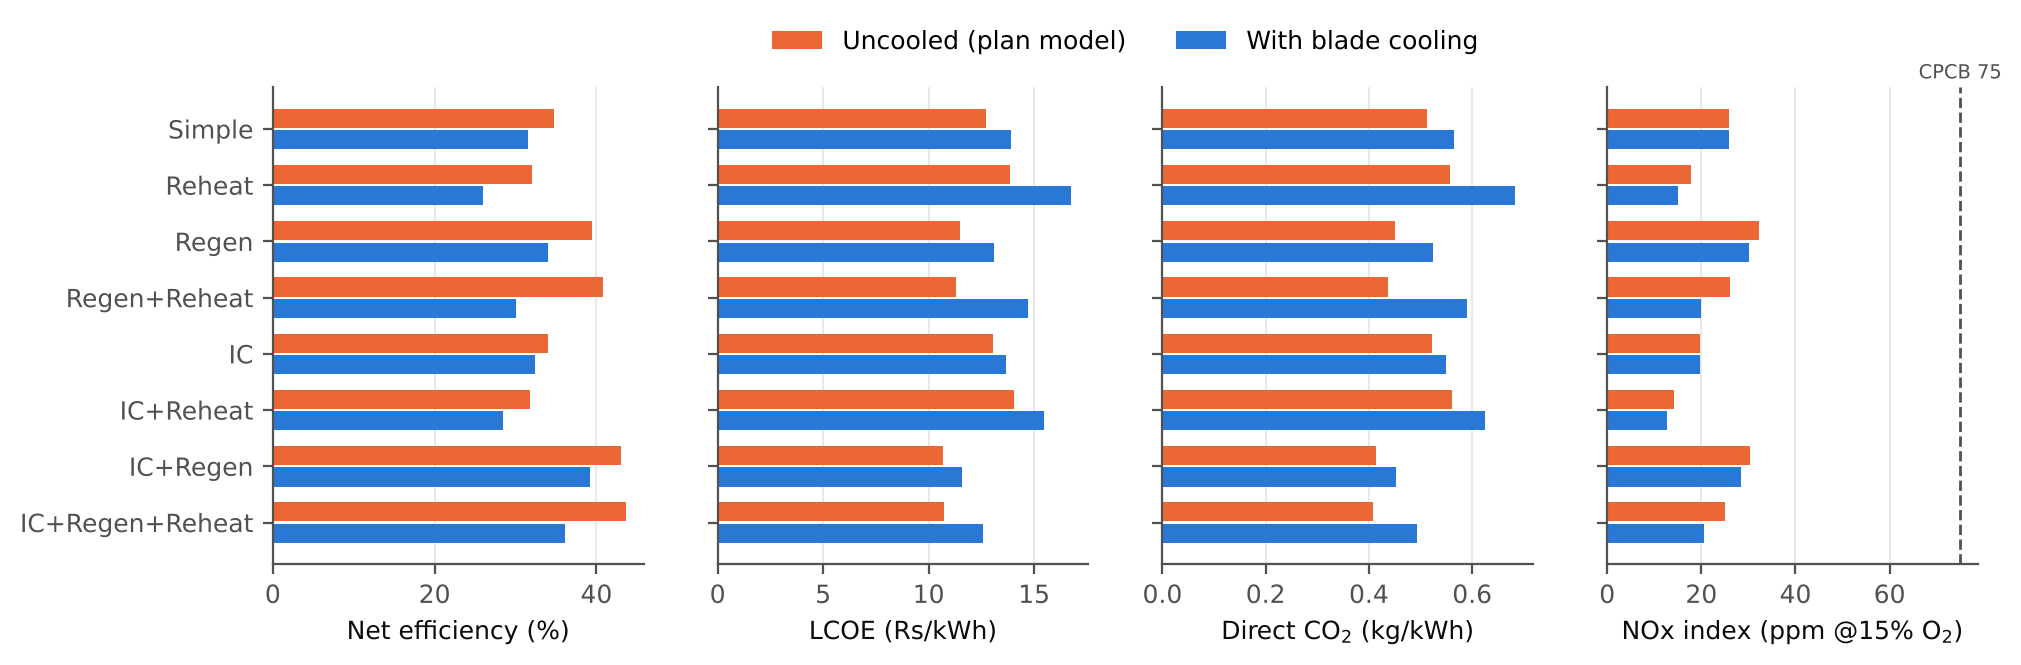
\includegraphics[width=\textwidth]{fig_candidate_configs.png}
\caption{Candidate layouts: uncooled plan model against the cooled integrated model.}\label{fig:cand}\end{figure*}
\begin{figure}[!t]\centering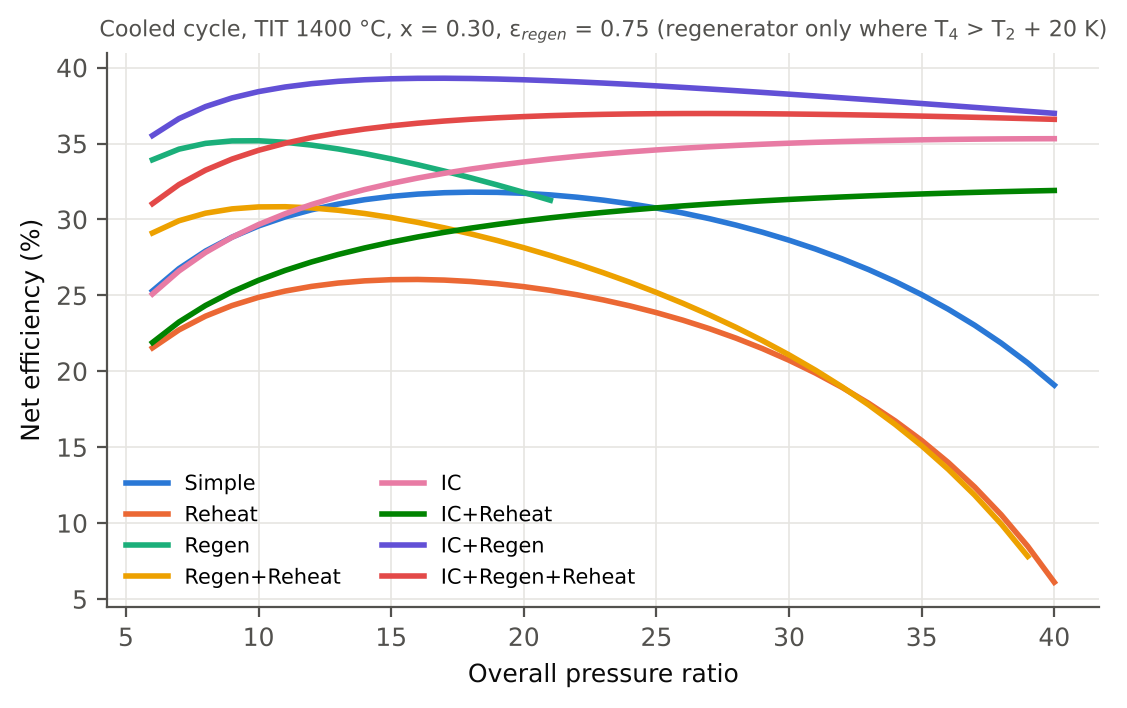
\includegraphics[width=\columnwidth]{fig_pr_sweep.png}
\caption{Net efficiency against pressure ratio for each layout (cooled; regenerative cycles shown only where $T_4-T_2\ge20$\,K).}\label{fig:pr}\end{figure}
\begin{figure}[!t]\centering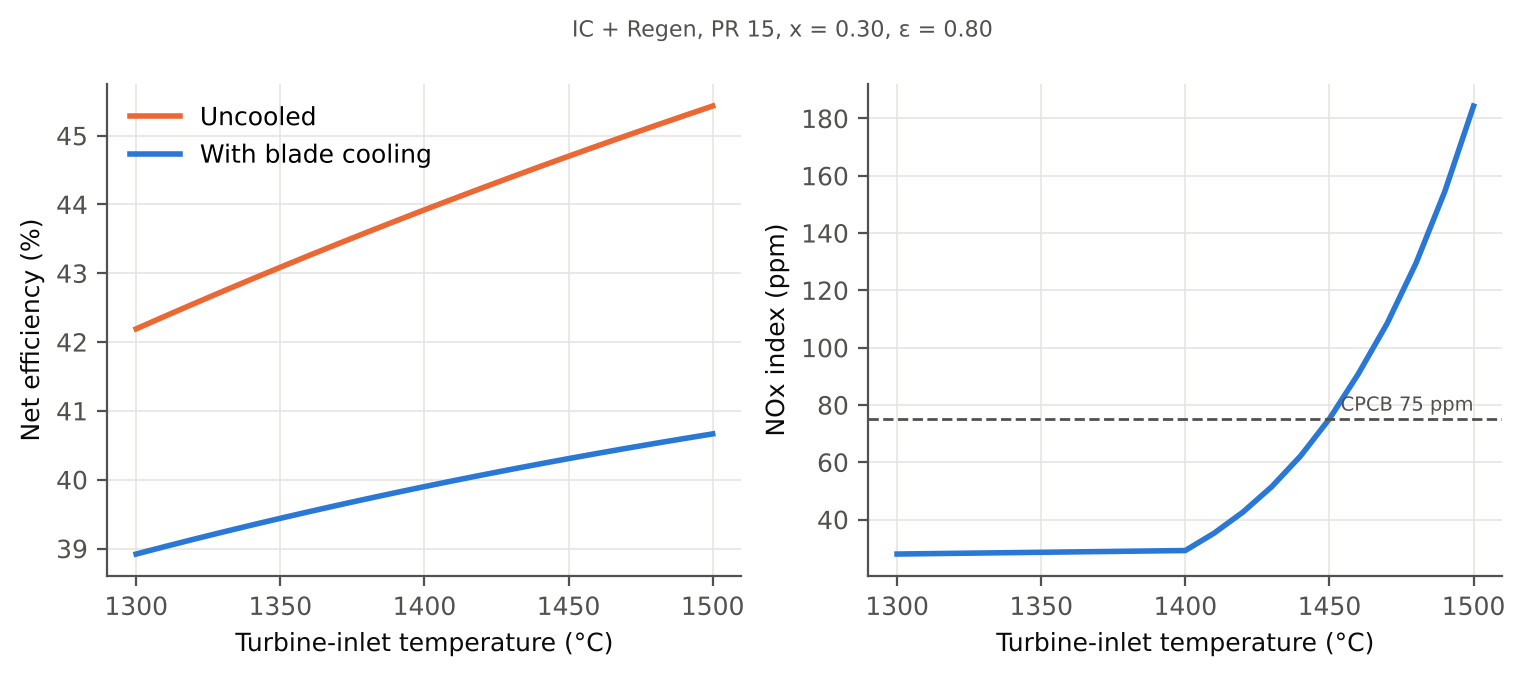
\includegraphics[width=\columnwidth]{fig_tit_tradeoff.png}
\caption{TIT trade-off on IC+Regen ($r_p=15$, $x=0.3$): small efficiency gain with cooling (left); NOx index crosses the CPCB limit near 1450\,\textdegree C (right).}\label{fig:tit}\end{figure}

\subsection{Overall exergy balance}
\begin{table*}[!t]\centering\caption{Plant Exergy Balance at 100\,MW (MW and \% of Fuel Exergy)}\label{tab:ex}
\scriptsize\input{\T{exergy.tex}}\end{table*}
Combustion is the largest irreversibility in every case, at about 34--35\% of the fuel exergy (Table~\ref{tab:ex}, Fig.~\ref{fig:ex}). It is fixed by the gap between the flame and the usable 1673\,K, not by the fuel. The final design raises $\Psi$ from 30.3\% (cooled baseline) to \finPsi\%, mainly by halving the stack loss through regeneration. The intercooler (3.4\%) and regenerator (1.8\%) add new losses, but these are small by comparison.
\begin{figure*}[!t]\centering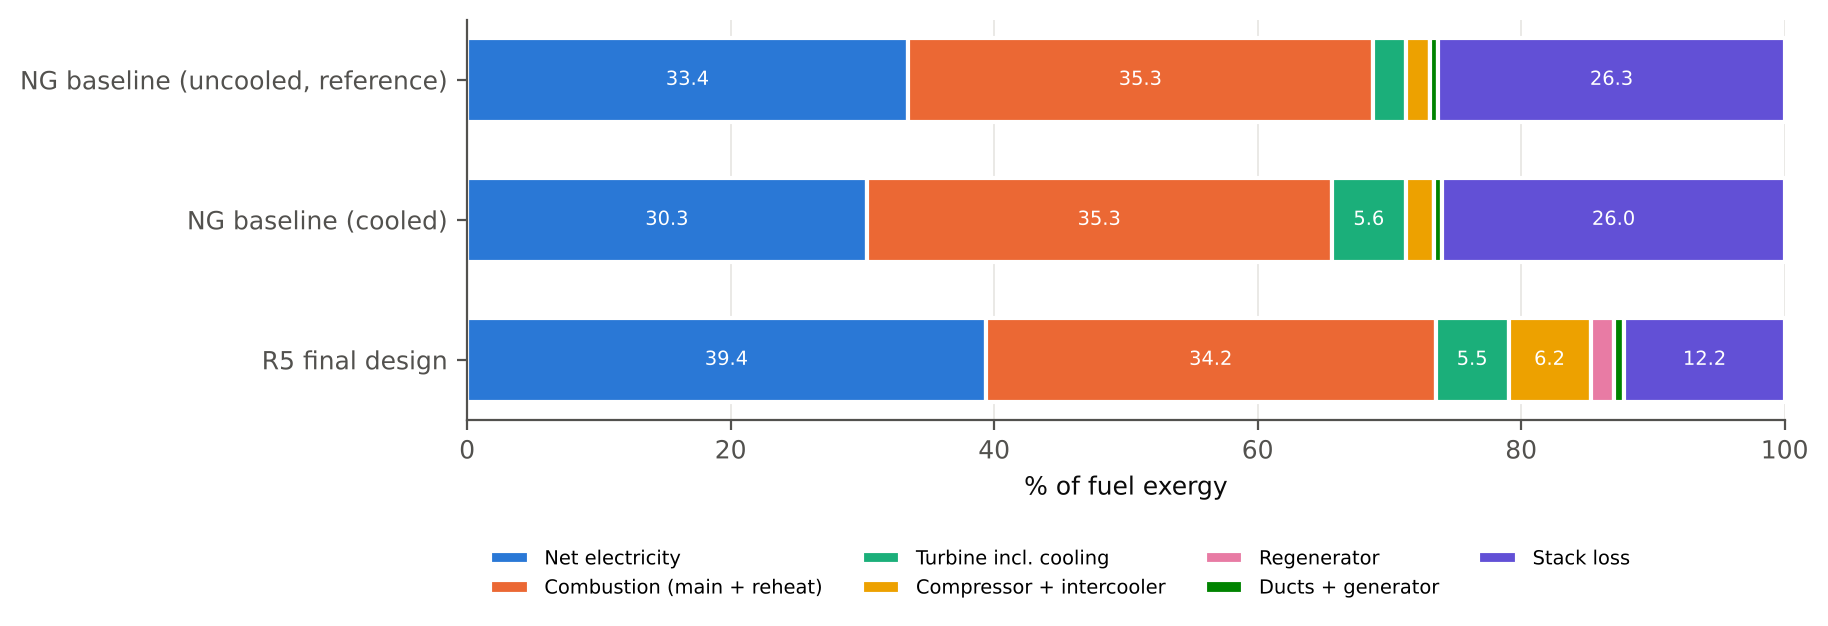
\includegraphics[width=0.8\textwidth]{fig_exergy_balance.png}
\caption{Destination of the fuel exergy: plan baseline, cooled baseline and final design.}\label{fig:ex}\end{figure*}

\subsection{Multi-objective optimisation}
\emph{Formulation.} Variables: $r_p\in[8,30]$, TIT $\in[1300,1500]$\,\textdegree C, $x\in[0,1]$, $\varepsilon\in[0.50,0.85]$, giving 8 on/off cases. Objectives: $\max\eta_{net}$; $\min$ exergy destruction (MJ/kWh); $\min$ LCOE; $\min$ CO$_2$; $\min$ NOx. Constraints: NOx $\le75$\,ppm; $FI\le2$; $T_5\le1050$\,K; reheat $x\le x_{max}(r_p)$; regenerator approaches $\ge$20\,K; TIT $\le1500$\,\textdegree C.

\emph{Algorithm.} NSGA-II \cite{deb} with constrained domination, SBX crossover ($\eta_c=15$) and polynomial mutation ($\eta_m=20$), population 100, 150 generations, run once per layout (120\,800 evaluations). pymoo was not available, so it was implemented in NumPy. A \nScan-point grid supplies the constraint statistics. The feasible results were merged and filtered to the global five-objective non-dominated set.

\begin{table}[!t]\centering\caption{Constraint Filtering (Grid Scan) and Pareto Membership}\label{tab:feas}
\scriptsize\input{\T{feasibility.tex}}\\[4pt]\input{\T{feas_config.tex}}\end{table}
Flashback removes the most designs (high-$x$ premixed blends), followed by reheat autoignition and NOx (Table~\ref{tab:feas}). \emph{Only intercooled layouts reach the Pareto set.} The four Pareto plots required by the brief are in Fig.~\ref{fig:pareto}. LCOE against CO$_2$ is the sharpest conflict, because along the front each step of hydrogen buys CO$_2$ at an almost constant price. Efficiency and LCOE do not conflict at fixed $x$: the most efficient IC+Regen designs are also the cheapest.
\begin{figure*}[!t]\centering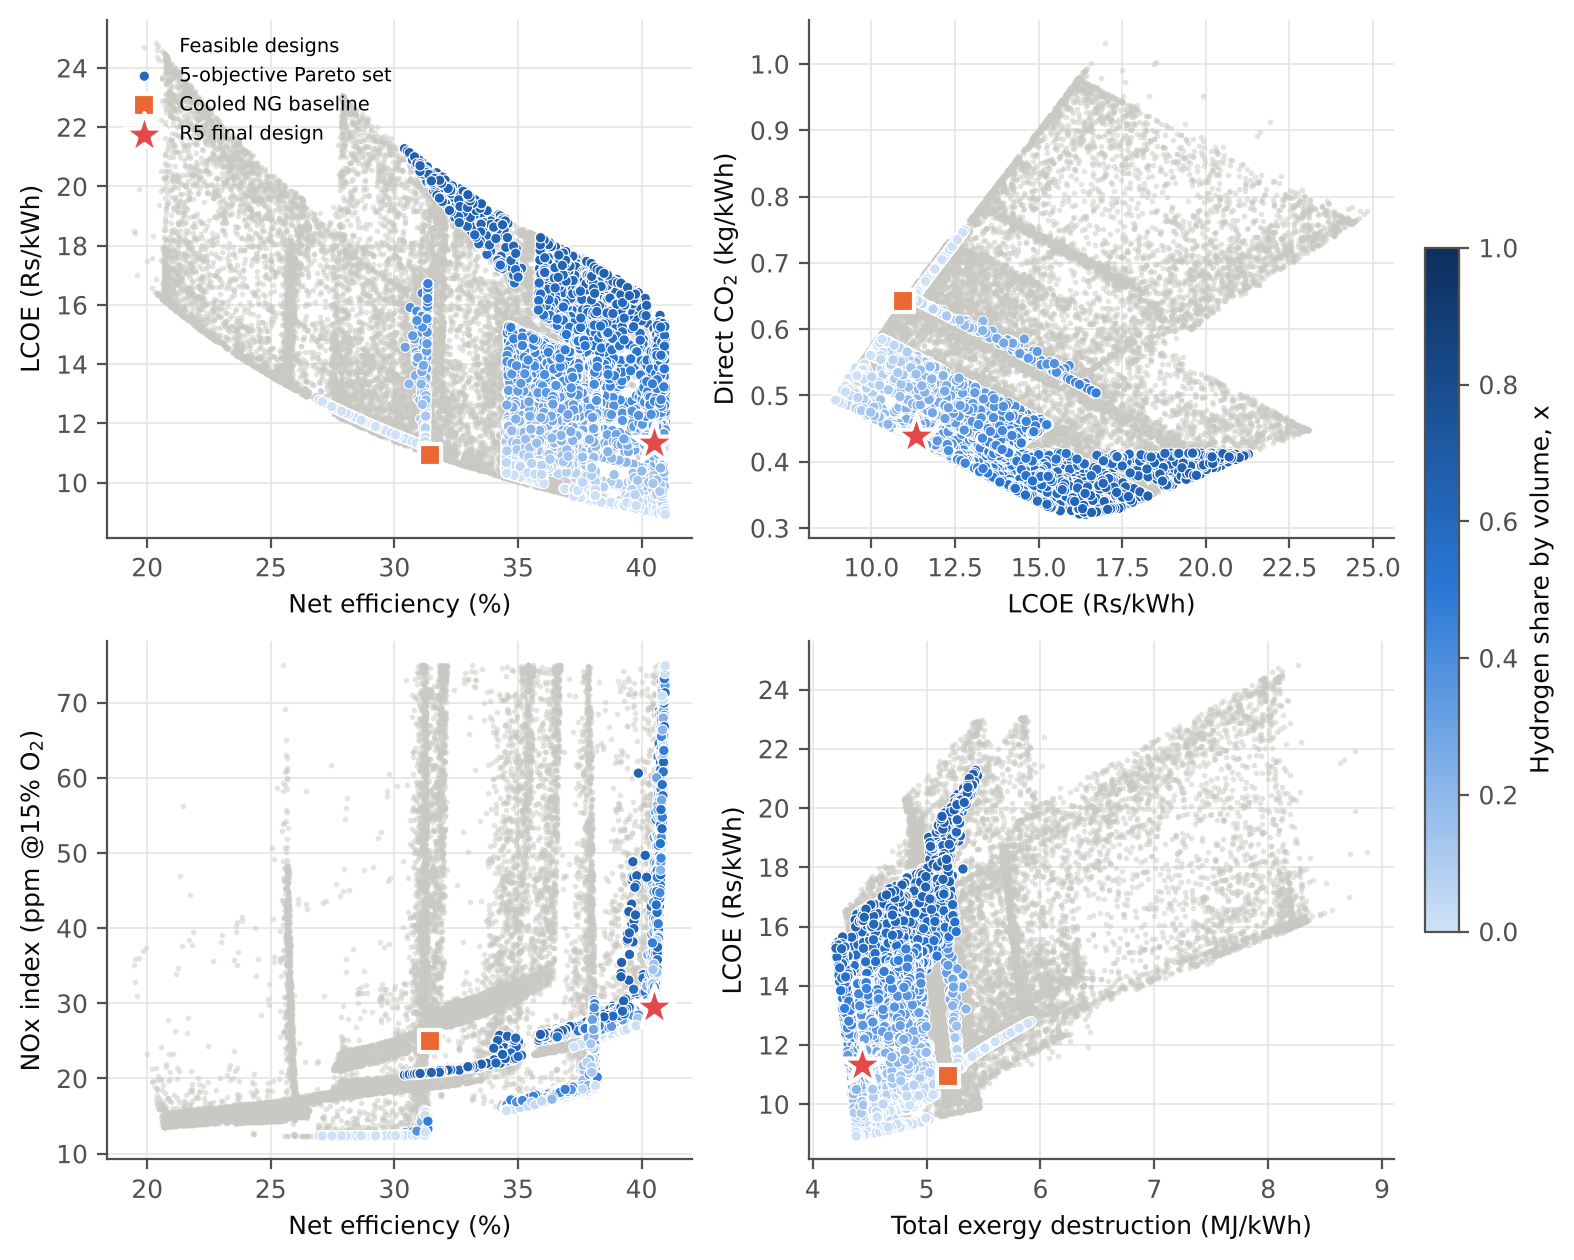
\includegraphics[width=0.86\textwidth]{fig_pareto_fronts.png}
\caption{Pareto deliverables: efficiency--LCOE, LCOE--CO$_2$, efficiency--NOx, exergy destruction--LCOE. Grey: feasible designs; coloured: five-objective Pareto set (shade = $x$); square: cooled NG baseline; star: final design.}\label{fig:pareto}\end{figure*}

%==================================================================================
\section{Selection of the Final Design}\label{sec:sel}
\subsection{TOPSIS}
\begin{table*}[!t]\centering\caption{TOPSIS Winners for Two Normalisations and Five Weight Sets (LCOE Rs/kWh, CO$_2$ kg/kWh, NOx ppm)}\label{tab:topsis}
\scriptsize\input{\T{topsis.tex}}\end{table*}
TOPSIS \cite{topsis} was applied to the Pareto set (Table~\ref{tab:topsis}). The winner depends on the \emph{normalisation}. With vector normalisation, the NOx index, which varies by a large relative amount (12--75\,ppm), dominates, and every weight set picks the low-NOx reheat design. With min-max normalisation, four of five weight sets pick IC+Regen.

\subsection{Reasoned trade-off}
\begin{table}[!t]\centering\caption{Head-to-Head of the Equal-Weight Winners}\label{tab:h2h}
\scriptsize\adjustbox{max width=\columnwidth}{\input{\T{headtohead.tex}}}\end{table}
The decision rule was fixed before the comparison: \emph{prefer the candidate better on the majority of objectives, provided its NOx keeps a one-third margin to the CPCB limit ($\le50$\,ppm)}. Design B (IC+Regen) is better on four of five objectives (Table~\ref{tab:h2h}): +2.6 points of efficiency, $-$0.18\,MJ/kWh, $-$\Rs0.77/kWh and $-$6\% CO$_2$. A's only advantage is an 11\,ppm lower NOx index, and that index is calibrated and relative. B also has practical advantages:
\begin{itemize}
\item no reheat combustor, so no autoignition-stabilised hydrogen flame (R2's limit would have to be extrapolated to $r_p=30$);
\item \Rs50\,crore less hardware and no second cooled turbine;
\item operation at $r_p=16$, inside the team's validated range, rather than on the $r_p=30$ search bound.
\end{itemize}

\subsection{Why the other layouts were rejected}
\begin{table*}[!t]\centering\caption{Best Feasible Design of Each Layout at $x=0.30$ (Equal-Weight Min-Max TOPSIS Over the Feasible Set) and the Reason It Was Not Chosen}\label{tab:why}
\scriptsize\input{\T{why_not.tex}}\end{table*}
To keep the comparison about the cycle alone, Table~\ref{tab:why} holds the hydrogen share at 0.30 and shows the best design of every layout. Layouts without regeneration lose a quarter of the fuel exergy in the stack. Layouts without intercooling need more coolant and leave a smaller regeneration margin. Every reheat layout pays for a second cooled turbine. IC+Regen+Reheat is the only close competitor, and it loses on four objectives.

\subsection{Choice of hydrogen share}
\begin{table}[!t]\centering\caption{Hydrogen Share on the Final Cycle}\label{tab:h2}
\scriptsize\adjustbox{max width=\columnwidth}{\input{\T{h2share.tex}}}\end{table}
On the chosen cycle, efficiency is almost independent of $x$ (Table~\ref{tab:h2}), as the brief anticipated. LCOE rises by about \Rs1/kWh for each 0.1 of $x$, CO$_2$ falls 4--5\% per 0.1, and flashback rules out $x>0.6$ with a tier-B premixer. Equal weighting gives $x=0.30$, which also stays in R2's tier A--B boundary hardware ($FI=1.29$). The same $x$ is selected at hydrogen prices of \Rs280, 350 and 400/kg (Table~\ref{tab:rob}).

%==================================================================================
\section{Final Design}\label{sec:final}
\begin{table}[!t]\centering\caption{State Points of the Final Design}\label{tab:states}
\scriptsize\adjustbox{max width=\columnwidth}{\input{\T{final_states.tex}}}\end{table}
\begin{table}[!t]\centering\caption{Final Design Against the Baselines}\label{tab:perf}
\scriptsize\adjustbox{max width=\columnwidth}{\input{\T{final_perf.tex}}}\end{table}
\begin{figure}[!t]\centering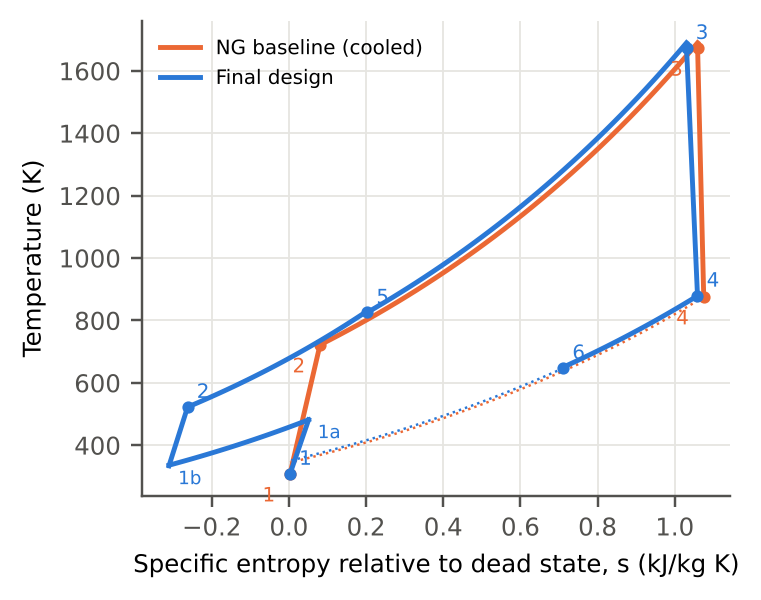
\includegraphics[width=\columnwidth]{fig_ts_diagram.png}
\caption{T--s diagram (constant-$c_p$ states): cooled NG baseline against the final design. Intercooling (1a--1b) and air preheat (2--5) are visible; dotted lines close the open cycle through the environment.}\label{fig:ts}\end{figure}

The selected plant (Tables~\ref{tab:states}--\ref{tab:perf}, Fig.~\ref{fig:ts}) draws \finMair\,kg/s of air and \finMfuel\,kg/s of blend, of which \finMh\,kg/s is H$_2$. Eight hours of storage holds \finStore\,t of H$_2$. The regenerator recovers \finQrg\,MW and preheats combustor air to \finTfive\,K, well below the 1050\,K autoignition limit. It needs about \finArea\,m$^2$ of surface. The stack leaves at \finTsix\,K. The flashback index is \finFI, within a tier-B premixer. All constraints are met with margin, and no design in the feasible set dominates it.

\begin{table}[!t]\centering\caption{Capital Cost of the Final Design}\label{tab:capex}
\scriptsize\adjustbox{max width=\columnwidth}{\input{\T{capex.tex}}}\end{table}
\begin{table}[!t]\centering\caption{LCOE Build-Up}\label{tab:lcoe}
\scriptsize\adjustbox{max width=\columnwidth}{\input{\T{lcoe_parts.tex}}}\end{table}

\emph{Economics and environment.} Capital is \Rs\finCapex\,crore (Table~\ref{tab:capex}) and fuel is \fuelShare\% of LCOE (Table~\ref{tab:lcoe}). Against the cooled baseline, CO$_2$ falls by \dCOpct\% for +\dLpct\% LCOE (\Rs\abateTot/t on average). This average hides two very different contributions:
\begin{itemize}
\item the \emph{cycle} improvement alone (same cycle on natural gas: \ngCO\,kg/kWh, \Rs\ngLCOE/kWh) removes \dCOcyclepct\% of the CO$_2$ at \emph{negative} cost;
\item the 30\% blend adds the rest at about \Rs\abateHtwo/t, consistent with R2's \Rs36\,000--44\,000/t.
\end{itemize}
Below about \Rs\parityPrice/kg of hydrogen, the final design is cheaper than the cooled baseline.

\subsection{What each role gives up}
\begin{table*}[!t]\centering\caption{Each Role's Individually-Best Value in the Feasible Set Against the Final Design}\label{tab:roles}
\scriptsize\input{\T{roles.tex}}\end{table*}
Table~\ref{tab:roles} lists each role's individually-best value and what the final design gives up against it.
\begin{itemize}
\item \textbf{R1} accepts a higher component exergy destruction (6.2\% of fuel exergy against a 1.2\% best), because the intercooler rejects heat. The return is less coolant and more regeneration.
\item \textbf{R2} gives up NOx (29.6 against a 12.4\,ppm best) and its climate optimum $x=1$, which is infeasible on flashback.
\item \textbf{R3} keeps TIT at 1400\,\textdegree C instead of its maximum-efficiency 1500\,\textdegree C, which breaks the NOx limit. It gives up reheat's 36\% higher specific work.
\item \textbf{R4} reaches 12.2\% stack loss, close to its 11.6\% best, at the upper screening effectiveness.
\item \textbf{R5}: efficiency is within 0.5 points of the best feasible. The \Rs2.4/kWh above the cheapest feasible design is the price of the blend.
\end{itemize}
Run through the cooled integrated model, R2's uncooled stand-in falls to 35.5\%, and R3's 1500\,\textdegree C case violates NOx (Table~\ref{tab:rc}).
\begin{table}[!t]\centering\caption{Subsystem Candidates in the Integrated Model}\label{tab:rc}
\scriptsize\adjustbox{max width=\columnwidth}{\input{\T{role_cands.tex}}}\end{table}

\subsection{Sensitivity and robustness}
\begin{figure}[!t]\centering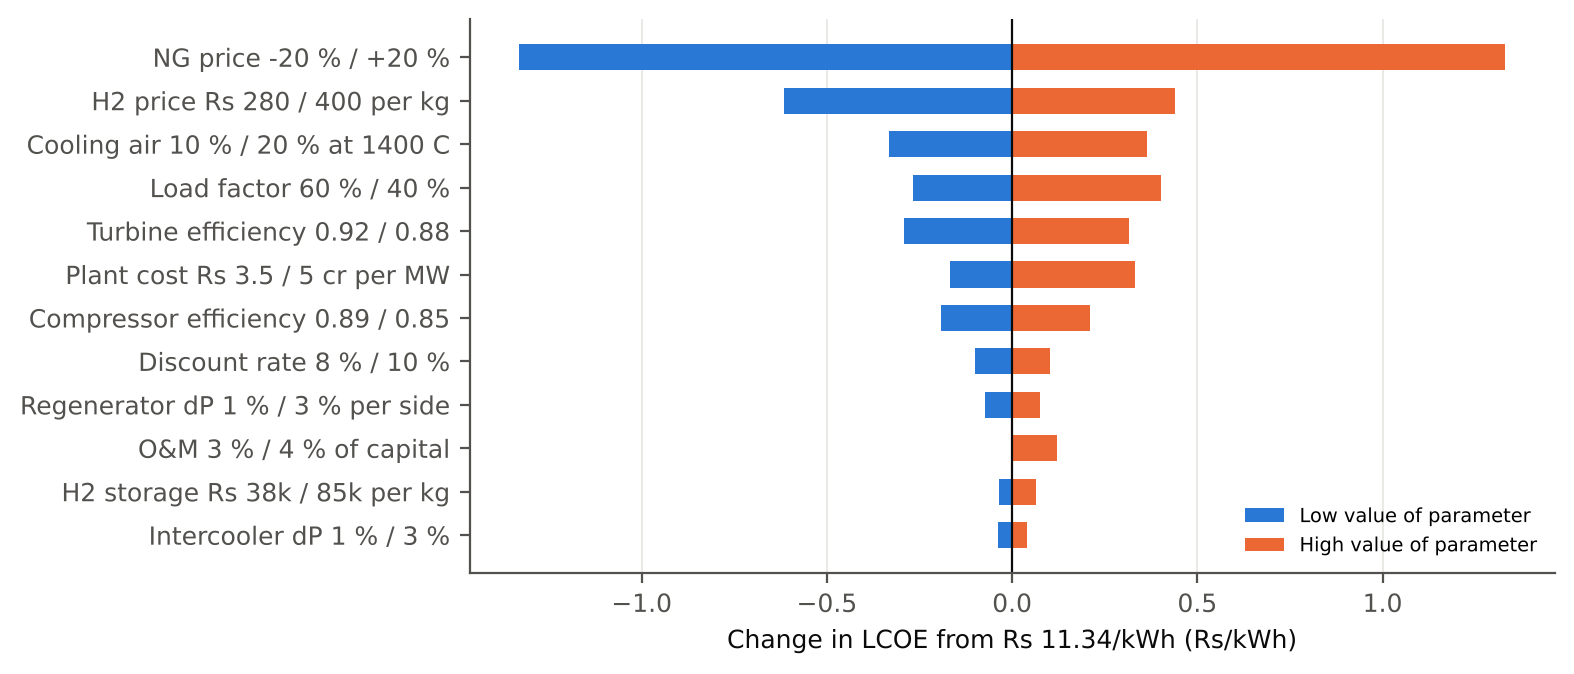
\includegraphics[width=\columnwidth]{fig_tornado.png}
\caption{One-at-a-time LCOE sensitivity of the final design. It remains feasible in every case.}\label{fig:tor}\end{figure}
\begin{figure*}[!t]\centering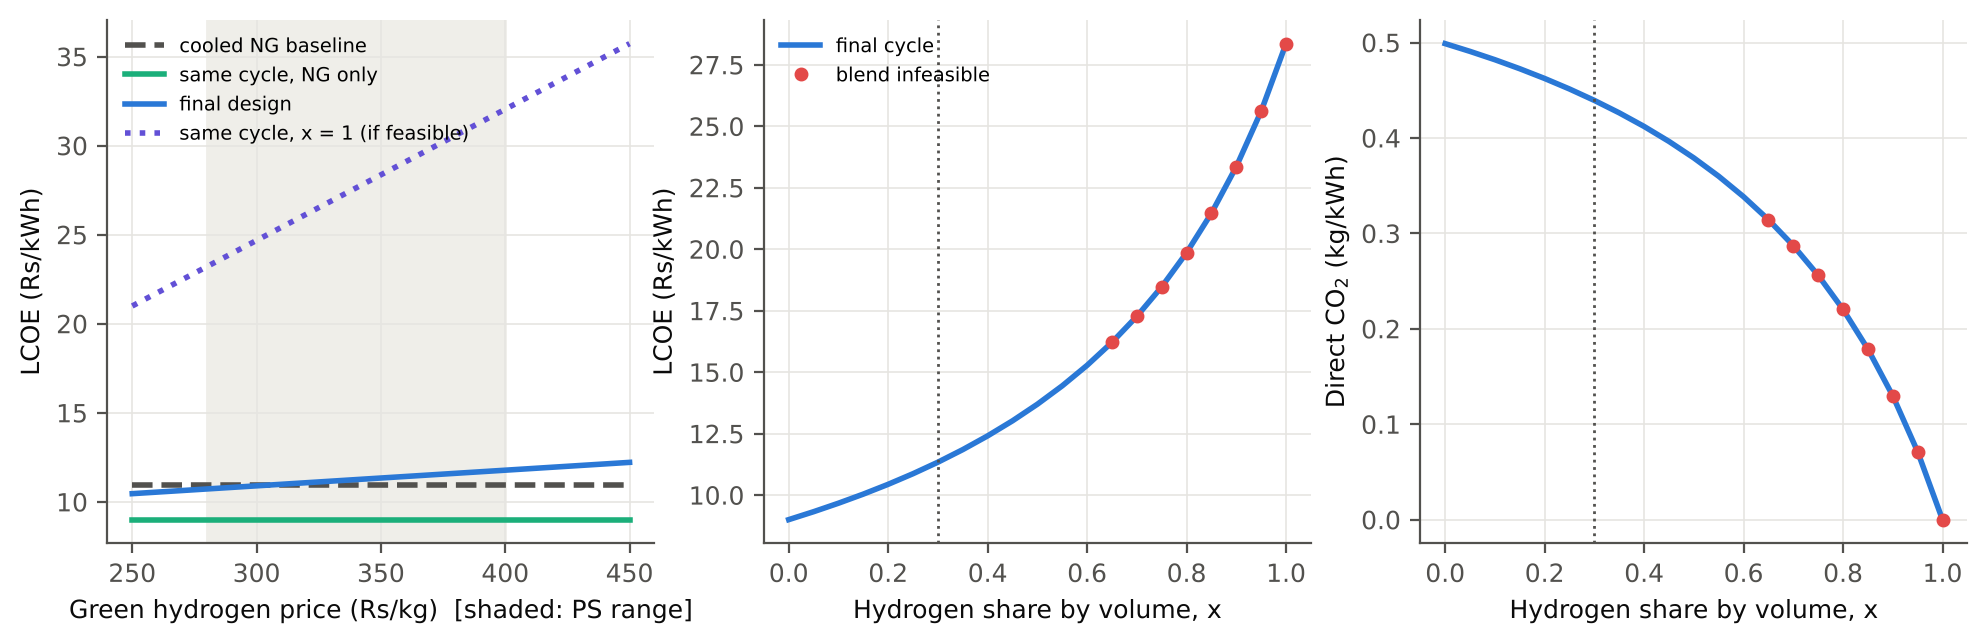
\includegraphics[width=0.9\textwidth]{fig_h2_price_share.png}
\caption{LCOE against hydrogen price (left); LCOE (centre) and CO$_2$ (right) against hydrogen share on the final cycle. Red markers: blends that break the flashback limit.}\label{fig:h2}\end{figure*}
\begin{table}[!t]\centering\caption{Robustness of the Selection to Hydrogen Price}\label{tab:rob}
\scriptsize\adjustbox{max width=\columnwidth}{\input{\T{robustness.tex}}}\end{table}
The natural-gas price ($\pm$20\%: $\pm$\Rs1.3/kWh) and the hydrogen price (\Rs280--400/kg: \Rs\lcoeLo--\lcoeHi/kWh) dominate (Fig.~\ref{fig:tor}, Fig.~\ref{fig:h2}). Among the engineering assumptions, the cooling-air fraction and turbine efficiency each move efficiency by about $\pm$1.5 points. Exchanger pressure losses, storage cost and the discount rate matter little. The selected configuration does not change across the hydrogen-price range (Table~\ref{tab:rob}).

%==================================================================================
\section{Discussion}
Three lessons emerged from the integration that no single subsystem study showed.
\begin{itemize}
\item \textbf{Couplings decide the ranking.} R1 saw intercooling as a modest compressor saving, R2 found reheat attractive without cooling, and R3 favoured the highest TIT. Combined, intercooling cuts coolant, cooling penalises reheat, and NOx caps TIT. The integrated answer differs from every subsystem optimum.
\item \textbf{Efficiency before hydrogen.} The cycle upgrade cuts CO$_2$ by \dCOcyclepct\% while saving money. Each further increment of hydrogen buys CO$_2$ at \Rs35\,000--40\,000/t at today's prices.
\item \textbf{Hydrogen is mostly a combustion problem.} The brief's claim is confirmed: efficiency changes by under one point from $x$ = 0 to 1. Flashback, autoignition and NOx, not the thermodynamics, limit the blend.
\end{itemize}

\section{Limitations}
\begin{itemize}
\item The constant-$c_p$ model (plan requirement) overstates fuel use by about 2.4\% against Cantera.
\item The cooling model is semi-empirical and calibrated by assumption. Real reheat machines cool the LP turbine with lower-pressure bleed and fire it below TIT, which would soften the reheat penalty.
\item The NOx index is calibrated (25\,ppm anchor) and relative. The primary-zone rule above 1400\,\textdegree C and the NOx surrogate are team assumptions. The CPCB limit is taken from a secondary source and should be checked against the Gazette.
\item Capital costs are percentage allowances with no scale credit. Storage cost uses US DOE tank data, and O\&M is held at 3\% for hydrogen.
\item Intercooler $\varepsilon$ is fixed at 0.85, exchanger losses at 2\%, and the reheat split as in R2. TOPSIS weights are judgements; the choice was checked across 10 weight and normalisation combinations.
\item CO$_2$ is direct only. With grey hydrogen, the blend would add no CO$_2$ benefit.
\end{itemize}

\section{Conclusion}
The five subsystem studies were combined into one validated cycle model whose exergy balance closes. It reproduces the plan's reference baseline and every subsystem hand-off. Five-objective NSGA-II with constraint filtering, TOPSIS under two normalisations and a pre-stated trade-off rule select an \textbf{intercooled--regenerative gas turbine with no reheat, at $r_p=\finPR$, TIT \finTITC\,\textdegree C, $x=\finX$ by volume (\finE\% energy) and $\varepsilon=\finEps$}. It achieves $\eta_{net}=\finEta\%$, heat rate \finHR\,kJ/kWh, $\Psi=\finPsi\%$, LCOE \Rs\finLCOE/kWh, \finCO\,kg CO$_2$/kWh and a NOx index of \finNOx\,ppm, against \bcEta\%, \Rs\bcLCOE/kWh and \bcCO\,kg/kWh for the cooled natural-gas baseline. Reheat was rejected because, with realistic blade cooling, its second cooled turbine and its autoignition-stabilised hydrogen flame cost more than its lower NOx is worth. Deeper hydrogen blending needs cheaper green hydrogen and flashback-proof burners for $x>0.6$.

\section*{Code and Data Availability}
All code, input parameters, results (CSV) and figures, together with the subsystem reports, are in the team repository \url{\RepoURL}. Running \texttt{python run\_pipeline.py} regenerates every number, table and figure in this report.

\section*{Acknowledgment}
The team thanks the ME 306 course instructor for the problem statement, baseline data and four-week plan.

\footnotesize
\begin{thebibliography}{99}
\bibitem{ps} ``Problem 16 --- Hydrogen-fueled / hydrogen-blended gas turbine for decarbonized grid power: full problem statement,'' ME 306 Course Project, 2026.
\bibitem{plan} ``Problem 16: four-week team plan,'' ME 306 Course Project, 2026.
\bibitem{r1} Team R1, ``Compressor and intercooling,'' ME 306 Problem 16 subsystem report, 2026.
\bibitem{r2} Team R2, ``Combustor and fuel blend,'' ME 306 Problem 16 subsystem report, 2026.
\bibitem{r3} Team R3, ``Turbine and reheat,'' ME 306 Problem 16 subsystem report and code, 2026.
\bibitem{r4} Team R4, ``Regenerator and exhaust heat recovery,'' ME 306 Problem 16 subsystem report, 2026.
\bibitem{heywood} J.~B. Heywood, \emph{Internal Combustion Engine Fundamentals}. New York, NY, USA: McGraw-Hill, 1988, ch.~11.
\bibitem{lefebvre} A.~H. Lefebvre and D.~R. Ballal, \emph{Gas Turbine Combustion: Alternative Fuels and Emissions}, 3rd ed. Boca Raton, FL, USA: CRC Press, 2010.
\bibitem{lewis} B. Lewis and G. von Elbe, \emph{Combustion, Flames and Explosions of Gases}, 3rd ed. Orlando, FL, USA: Academic Press, 1987.
\bibitem{szargut} J. Szargut, D.~R. Morris and F.~R. Steward, \emph{Exergy Analysis of Thermal, Chemical and Metallurgical Processes}. New York, NY, USA: Hemisphere, 1988.
\bibitem{gri} G.~P. Smith \emph{et al.}, ``GRI-Mech 3.0.'' [Online]. Available: http://combustion.berkeley.edu/gri-mech/; D.~G. Goodwin \emph{et al.}, ``Cantera,'' https://cantera.org.
\bibitem{doe} US DOE Hydrogen and Fuel Cell Technologies Office, ``Onboard type IV compressed hydrogen storage system cost,'' Record 13010, 2013.
\bibitem{cpcb} ``Environmental regulations on thermal power stations: gas-turbine NOx standards'' (secondary summary of the MoEF notification), 2010. [Online]. Available: https://mypowerplants.blogspot.com/2010/10/environmental-regulations-on-tps.html
\bibitem{mhi1} Mitsubishi Heavy Industries, ``Development of next-generation 1650\,\textdegree C-class JAC gas turbine,'' \emph{MHI Tech. Rev.}, vol.~56, no.~3, 2019.
\bibitem{mhi2} S. Hada and K. Takata, ``High-efficiency gas turbine development applying 1600\,\textdegree C class J technology,'' \emph{MHI Tech. Rev.}
\bibitem{cam} University of Cambridge, Phase Transformations Group, ``Coatings for turbine blades.'' [Online]. Available: https://www.phase-trans.msm.cam.ac.uk/2003/Superalloys/coatings/
\bibitem{cmsx} K. Harris \emph{et al.}, ``CMSX-4 single-crystal superalloy turbine blades,'' Cannon-Muskegon Corp., ASME paper. [Online]. Available: https://core.ac.uk/download/357389784.pdf
\bibitem{asme} ``Tradeoff assessments for part load controlled cooling air in stationary gas turbines,'' \emph{J. Eng. Gas Turbines Power}, doi:10.1115/1.4048452.
\bibitem{ceas} ``Comparison of cooling-air estimation methods for gas turbines,'' \emph{CEAS Aeronaut. J.}, 2024, doi:10.1007/s13272-024-00776-0.
\bibitem{horlock} J.~H. Horlock, D.~T. Watson and T.~V. Jones, ``Limitations on gas turbine performance imposed by large turbine cooling flows,'' \emph{J. Eng. Gas Turbines Power}, vol.~123, pp.~487--494, 2001.
\bibitem{lienhard} J.~H. Lienhard IV and J.~H. Lienhard V, \emph{A Heat Transfer Textbook}, 6th ed. Cambridge, MA, USA: Phlogiston Press, 2024.
\bibitem{deb} K. Deb, A. Pratap, S. Agarwal and T. Meyarivan, ``A fast and elitist multiobjective genetic algorithm: NSGA-II,'' \emph{IEEE Trans. Evol. Comput.}, vol.~6, no.~2, pp.~182--197, 2002.
\bibitem{topsis} C.-L. Hwang and K. Yoon, \emph{Multiple Attribute Decision Making: Methods and Applications}. Berlin, Germany: Springer, 1981.
\end{thebibliography}
\normalsize

\appendix
\section*{Appendix: Assumptions Added by the Team Beyond the Brief}
\begin{table}[!h]\centering\scriptsize
\begin{tabular}{@{}p{2.5cm}p{2.3cm}p{3.0cm}@{}}\toprule Item & Value & Basis\\\midrule
Firing limit & 1500\,\textdegree C & G/H-class \cite{mhi1,mhi2}\\
Blade metal; $\eta_{cool}$ & 1150\,K; 0.70 & R3; \cite{cam,cmsx}\\
Coolant at 1400\,\textdegree C & 15\% of air & \cite{asme,ceas}, R3\\
H$_2$ share basis & volume & R2\\
NOx anchor; limit & 25\,ppm @1790\,K; 75\,ppm & R2; \cite{cpcb}\\
Flashback limit & $FI\le2.0$ & R2 tier B\\
Autoignition & $T_5\le1050$\,K; reheat $x_{max}(r_p)$ & R2\\
$\varepsilon_{IC}$; $\Delta p$ IC/regen & 0.85; 2\%/2\% & R1; R4 range\\
Regenerator cost & $\propto UA$ & R4\\
Hot-section cost & +4\%/100\,K & R3\\
H$_2$ storage & \Rs55\,000/kg, 8\,h & R2, \cite{doe}\\
Upstream CO$_2$ of H$_2$ & 0 (green) & team\\\bottomrule
\end{tabular}\end{table}
\end{document}
